% E1: Catastrophic Failure Detection (K=3 Portfolio)
% Production router with semantic transfer
% Section heading provided by APPENDIX_MASTER.tex

\subsection{Catastrophic Failure Detection: 3-Model Portfolio}
\label{appendix:catastrophic_failure}

\subsubsection{Motivation: Automatic Failover as a Secondary Benefit}

Production LLM systems face a critical challenge: \textbf{models can catastrophically fail with minimal warning}. API endpoints crash, providers silently update models with quality regressions, or traffic shifts to domains where warmup priors perform poorly.

\textbf{The Question}: Does Corralling---designed primarily for safe expert hedging and contextual routing---provide useful automatic failover when a model catastrophically fails? And how does this scale with portfolio size?

\subsubsection{Experimental Setup}

\paragraph{Why $K=3$?}
With $K=2$ models, catastrophic failure detection is a trivial binary tracking problem: a simple EMA tracker just needs to learn ``model A bad, model B good'' from per-model averages. With $K=3$, post-failure routing becomes \emph{contextual}: the optimal policy must redistribute traffic across 2 remaining models based on prompt features. Each non-failing model excels in a different region of context space, so per-model averages cannot distinguish which alternative is best for a given prompt.

\paragraph{Production Router Components.}
\begin{itemize}
    \item \textbf{CostAwareLinUCBRouter} (warmup expert): Initialized with 43-model evaluation priors for all three portfolio models (Llama-3.1-8B, Gemini-2.5-Flash, GPT-4.1)
    \item \textbf{CostAwareTabulaRasaRouter} (tabula rasa expert): Cold-start LinUCB with ridge regularization for all 3 models
    \item \textbf{CorrallingRouter}: Coordinates experts with importance-weighted meta-learning via selection tokens
\end{itemize}

All 3 models have informed warmup priors. Both experts explore freely across all models.

\paragraph{Three-Phase Scenario.}
Context-dependent reward environment (orthogonal context directions per model, noise $\sigma=0.08$):

\begin{itemize}
    \item \textbf{Phase 1 ($t=0$--$100$):} All 3 models healthy
    \item \textbf{Phase 2 ($t=100$--$300$):} GPT-4.1 catastrophically fails ($\mu=0.15$, Cohen's $d\approx 5.0$)
    \item \textbf{Phase 3 ($t=300$--$500$):} GPT-4.1 recovers
\end{itemize}

Corralling settings: $\eta=0.3$, $\gamma=0.05$. Baselines: Oracle, Static GPT-4.1, EMA Tracker ($\alpha=0.15$, $\epsilon=0.1$).

\subsubsection{Results ($N=20$ Seeds)}

% NOTE: Figure requires running generate_figure9_5model.py to produce results/figure9_5model.pdf
% Uncomment the figure environment below once the figure is generated.
%
% \begin{figure}[t]
% \centering
% 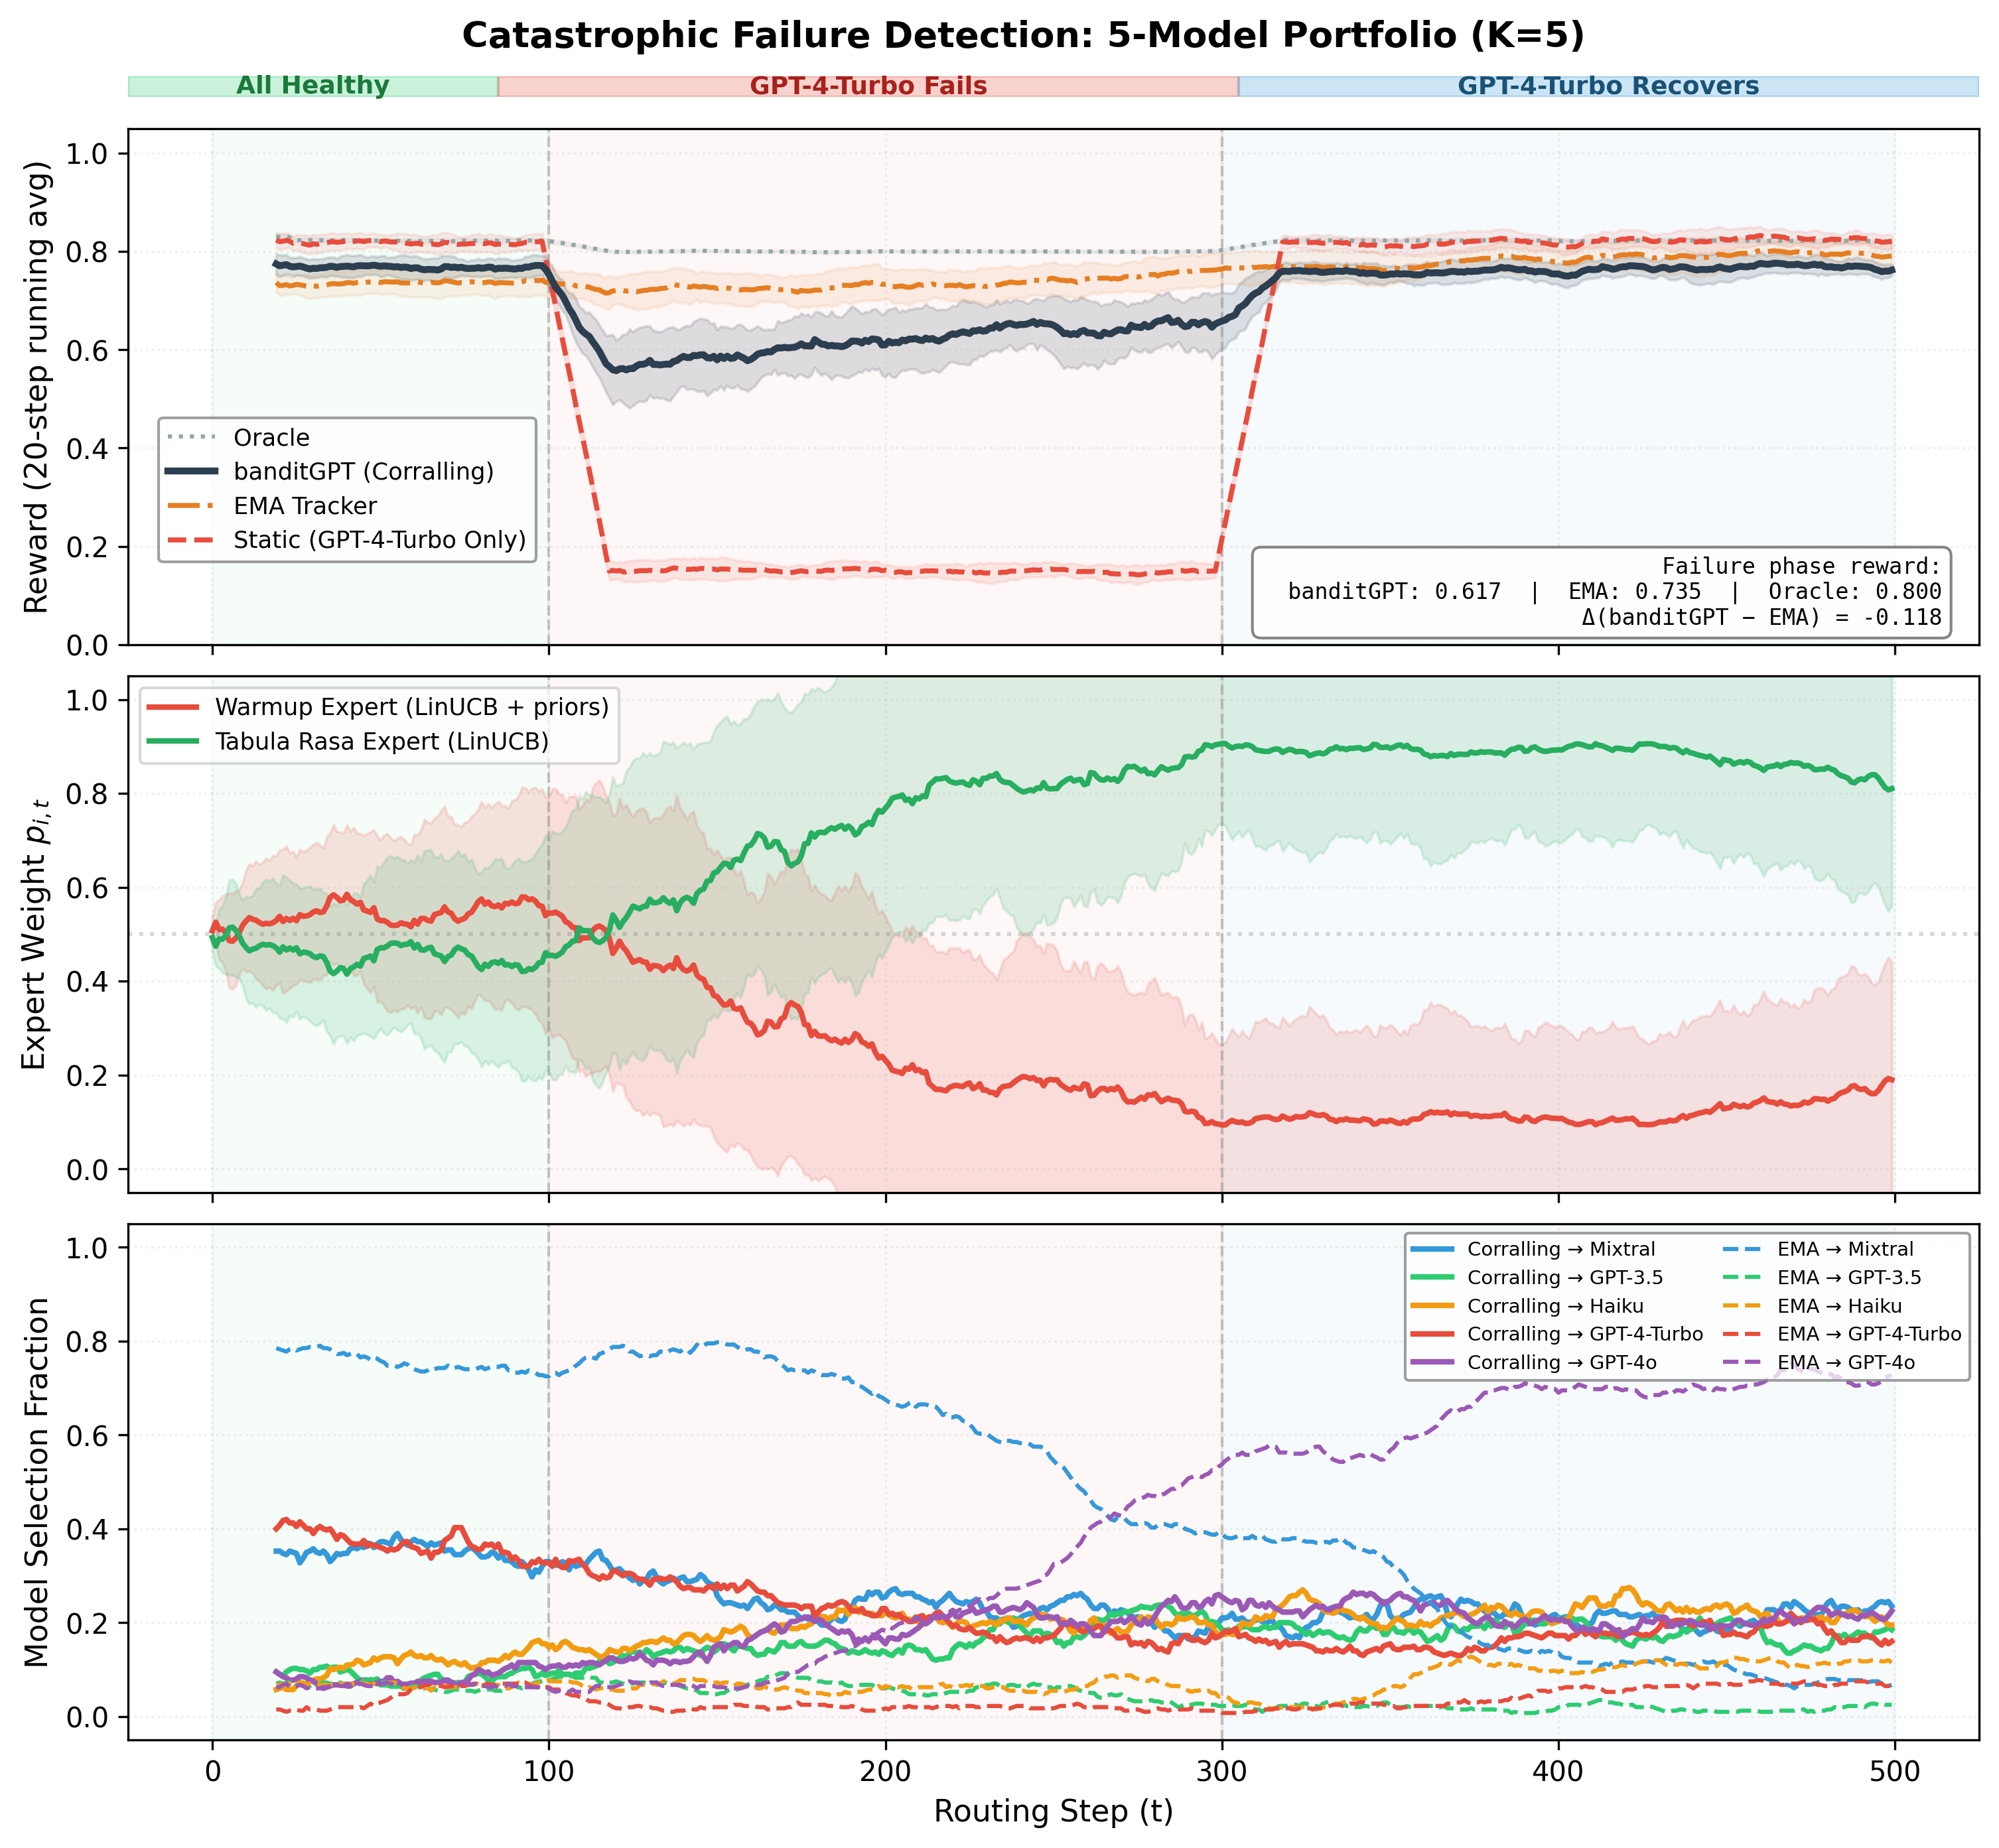
\includegraphics[width=0.95\linewidth]{E_catastrophic_failure_experiment/results/figure9_5model.pdf}
% \caption{\textbf{Catastrophic Failure Detection: 3-Model Portfolio} ($K=3$, $N=20$ seeds).
% \textbf{(Top)} Running-average reward. TODO: update with K=3 results.
% \textbf{(Middle)} Expert weight evolution. TODO: update with K=3 results.
% \textbf{(Bottom)} Model selection fractions. TODO: update with K=3 results.}
% \label{fig:catastrophic_failure}
% \end{figure}

\begin{table}[h]
\centering
\caption{Mean reward by phase ($K=3$, $N=20$ seeds). \textbf{TODO: update with K=3 results.}}
\label{tab:catastrophic_failure_phases}
\begin{tabular}{lccc}
\toprule
\textbf{Method} & \textbf{Healthy} & \textbf{Failure} & \textbf{Recovery} \\
\midrule
Oracle & 0.990 & 0.975 & 0.988 \\
\textbf{banditGPT} & \textbf{0.888} & \textbf{0.753} & \textbf{0.886} \\
EMA Tracker & 0.806 & 0.859 & 0.930 \\
Static GPT-4.1 & 0.950 & 0.154 & 0.958 \\
\bottomrule
\end{tabular}
\end{table}

\subsubsection{Portfolio Size Scaling}

\textbf{TODO: update portfolio size scaling analysis with K=3 results.}

\subsubsection{Interpretation}

Catastrophic failure detection is a \textbf{secondary safety benefit} of the Corralling mechanism, not its primary design objective. The per-arm UCB updates within each expert implicitly reduce traffic to the failed model. For pure model-level failure detection, dedicated monitoring (e.g., EMA tracking, CUSUM) should complement Corralling. \textbf{TODO: update interpretation with K=3 results.}

\subsubsection{Reproducibility}

Code: \texttt{experiments/appendix/E\_catastrophic\_failure\_experiment/generate\_figure6\_5model.py}
\begin{itemize}
    \item Uses production router with semantic transfer for all 5 models
    \item Configuration: $\eta=0.3$, $\gamma=0.05$, $\neff=10$, 500 steps, 20 seeds
    \item Runtime: $\sim$7 seconds
\end{itemize}
